\documentclass{article}

\usepackage{graphicx}
\usepackage{courier}
\usepackage{float}

\begin{document}


\begin{titlepage}
\begin{center}


{\huge \textbf{COS 314: Assignment III}}

\vspace{2cm}

{\Large Iwan de Jong}

\vspace{1cm}

{\large u22498037 \\ 
University of Pretoria} 

\vfill

\end{center}
\end{titlepage}

\tableofcontents

\section{Assignment-specific Parameters}
A seed value of 1 has been used.

\section{Pre-Processing}
For pre-processing, the data was normalised using the Min-Max method. Both the testing and training data were normalised using the same parameters. The values represented in the data were scaled to a range of 0 to 1.

\section{ANN Technical Specification}
\subsection{ANN Structure}
The ANN consists of 3 layers: an input layer, a hidden layer, and an output layer. 

The input layer consisted of 8 nodes, the hidden layer consisted of 5 nodes, and the output layer consisted of 1 node.
The output layer uses a sigmoid activation function, while the hidden layer uses a sigmoid activation function. It only has one output node, which is used to determine the output of the ANN (which is binary (either 0 or 1)).

It was then feed-forwarded through the network, and the error was back-propagated to adjust the weights.

When training, I also made the mushroom input random, so that it wouldn't converge to a local minimum.

In this ANN, 0 represented a non-edible (toxic) mushroom, while 1 represented an edible mushroom.

\subsection{Activation Function}
The activation function used is the sigmoid function. The sigmoid function is defined as:
\begin{equation}
    f(x) = \frac{1}{1 + e^{-x}}
\end{equation}

Likewise, the derivative of the sigmoid function is defined as:

\begin{equation}
    f'(x) = f(x) * (1 - f(x))
\end{equation}

I used the sigmoid function as it is a common activation function for binary classification problems, since it maps the output to a range of 0 to 1.

\subsection{Learning Rate}
The learning rate is set to 0.23. 

For this model, the parameter greatly affects the convergence of the model. I chose a learning rate of 0.23 as it provided the best results. I found that lower learning rates resulted in weaker results, while higher learning rates resulted in the model not converging.

\subsection{Stopping Condition}
The stopping condition is set to go 1000 epochs, regardless of improvement. I found that the model converged within 1000 epochs, and that the error rate did not improve significantly after this point.

\subsection{Additional Statistics}
\begin{verbatim}
    Statistics
    Precision: 0.742678
    Recall: 1.000000
    Accuracy: 0.796020
    F1 Score: 0.852341

    Output Statistics:
    Mean: 0.464287
    Variance: 0.000900
    Standard Deviation: 0.029995
    Range: 0.116922
\end{verbatim}

\subsection{Critical Analysis}
The ANN model had a great accuracy and good recall, but the precision was not good. As seen with the output, the variance is extremely low, which is not good, since the value of the output is binary, there should be a higher variance. The range is also very low, which is not good, as the output should be more varied. This will make it easy for the model to predict the output. 

Consequently, when the seed/initial weights are changed, the model will not perform as well, as the model is not generalised to perform well on unseen data.

Overall, it does have a good accuracy, and the mean is close to 0.5, which is good, as the output is binary.

\subsection{Graphical Representation}
The graphical representations obtained from `output.csv` are generated after each epoch (generated by ANN.cpp).
    \begin{figure}[H]
        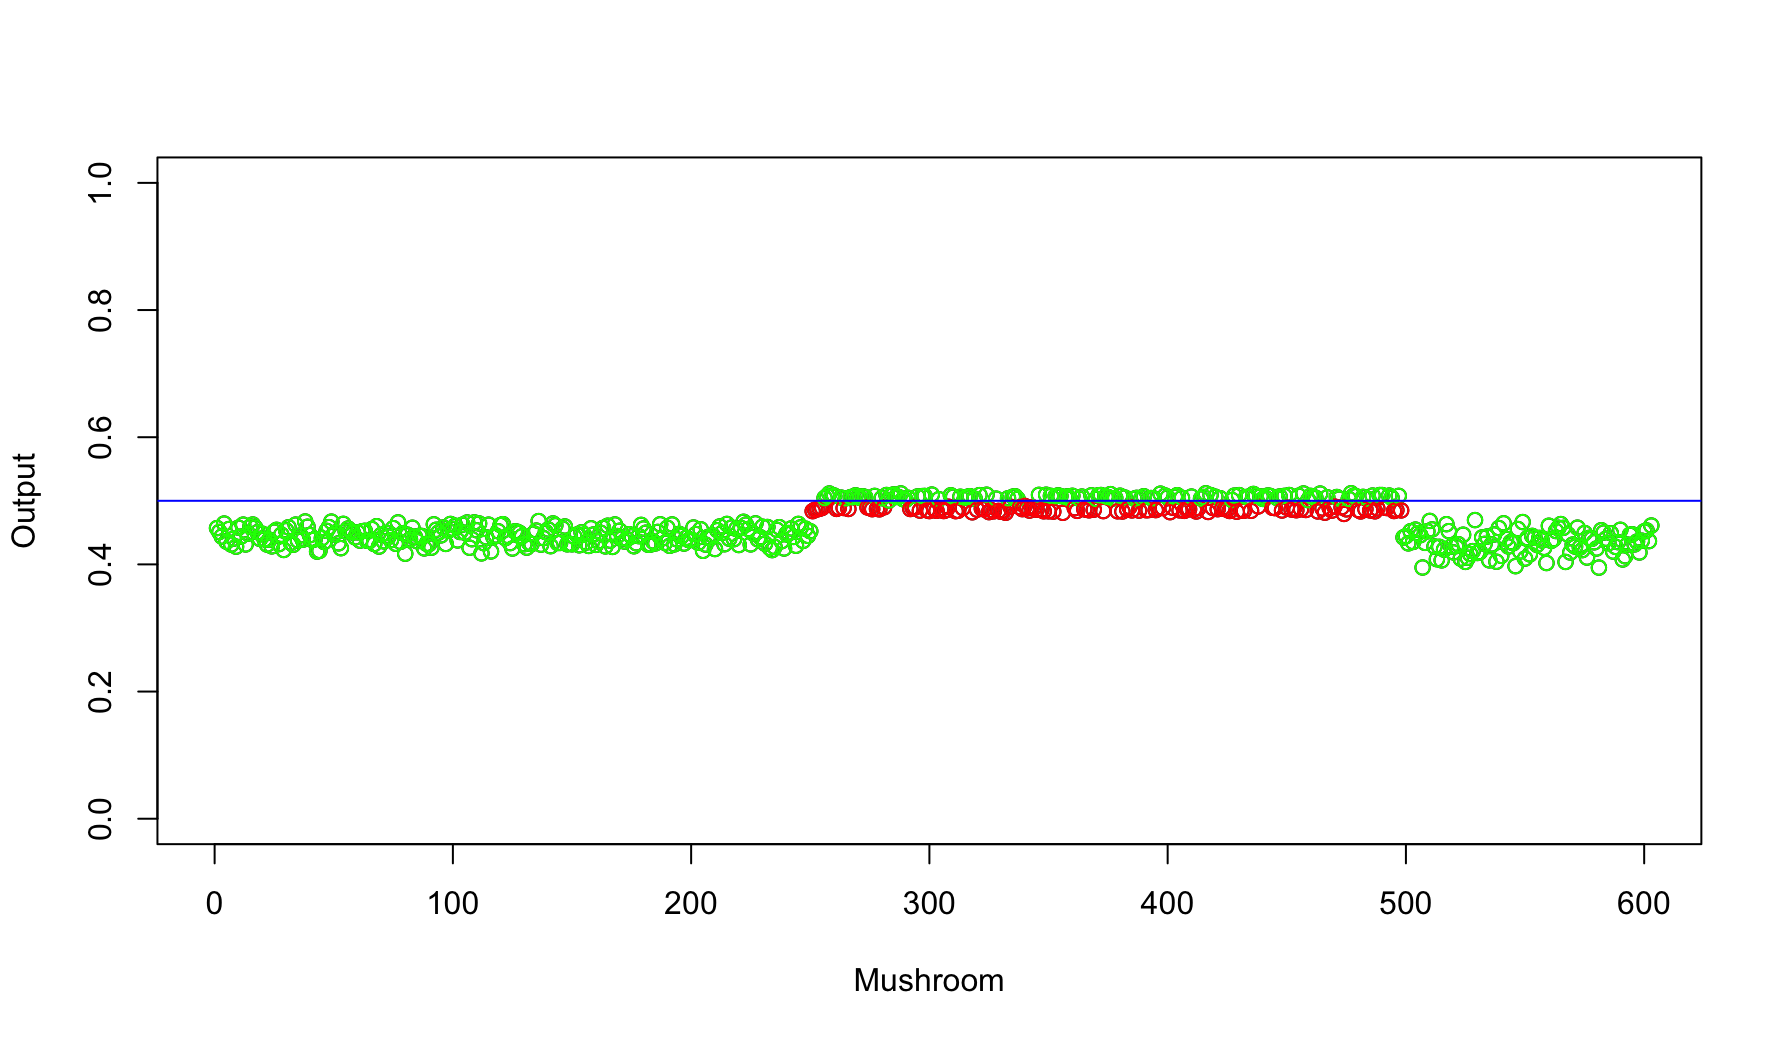
\includegraphics[width=\linewidth]{scatterplot.png}
        \caption{Scatterplot of the expected data versus the ANN output. The red dots represents errors.}
        \label{fig:ils}
    \end{figure}

    \begin{figure}[H]
        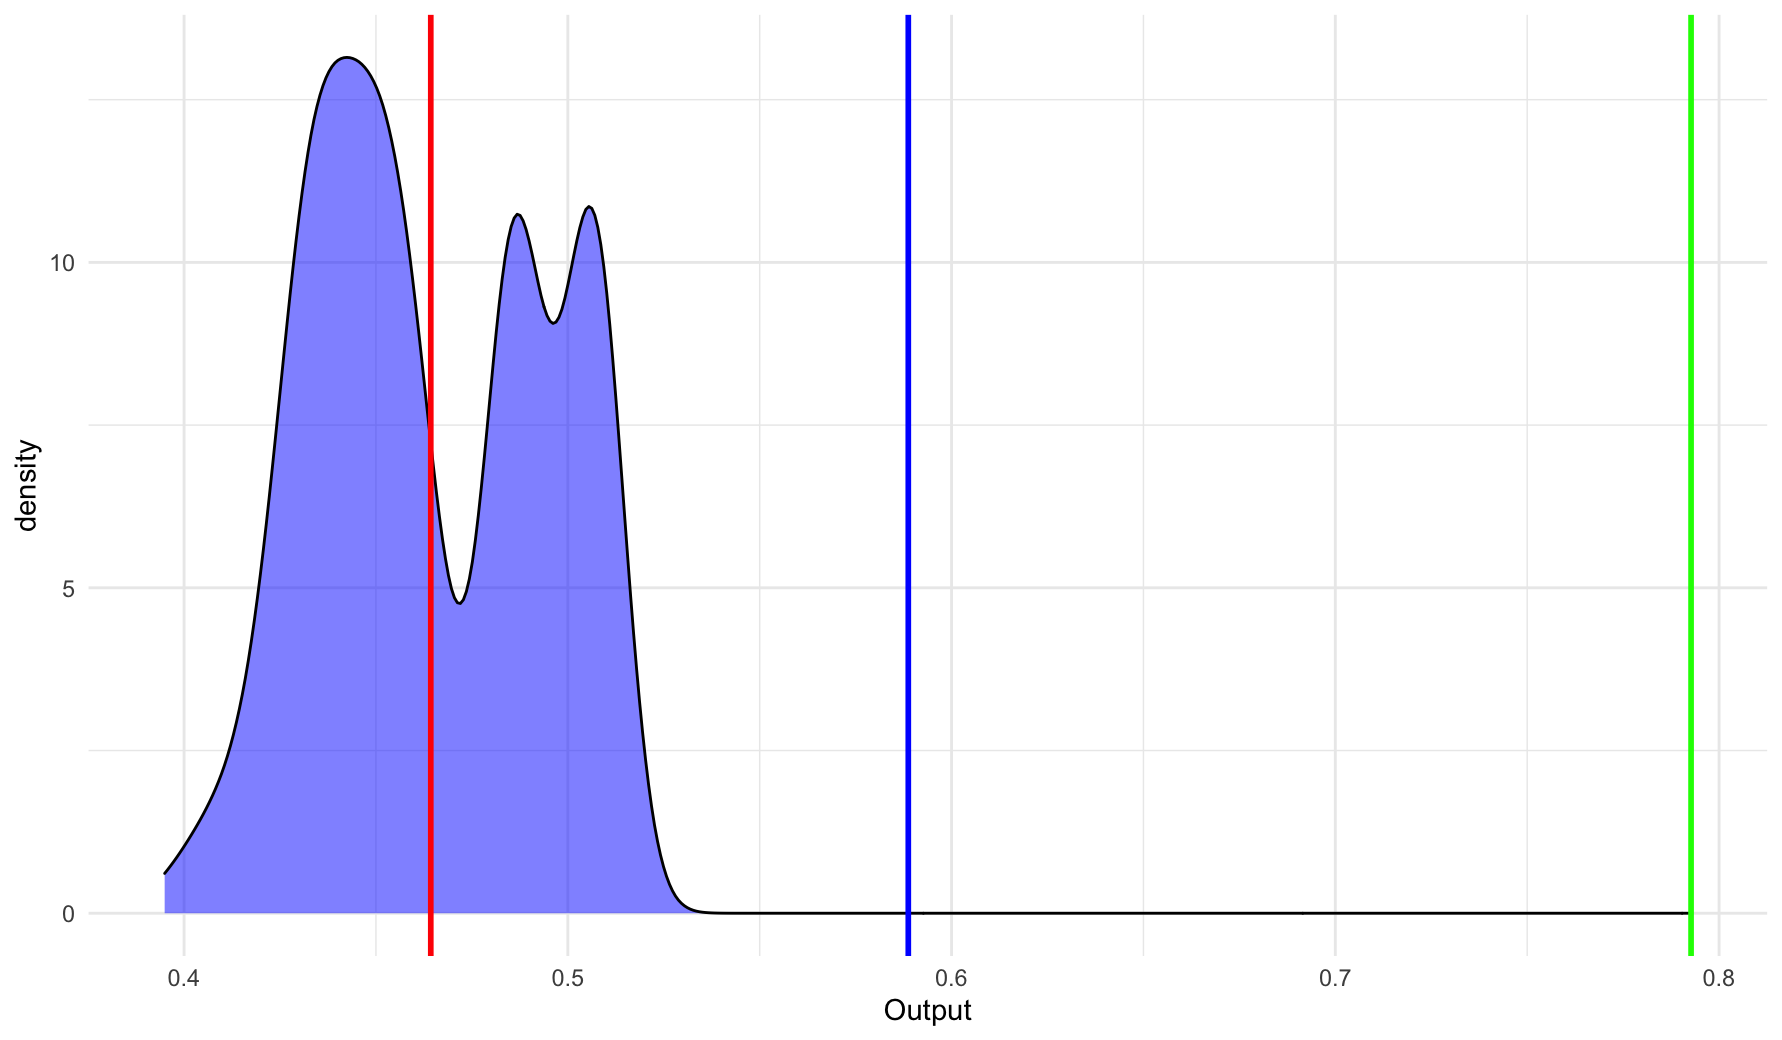
\includegraphics[width=\linewidth]{densityPlot.png}
        \caption{Density Plot of the ANN output. The red line gives the average output, the blue line gives the expected output, and the green line gives the actual output.}
        \label{fig:sa}
    \end{figure}

The graphical representations obtained from `error.csv` are generated after each epoch (generated by ANN.cpp).
    \begin{figure}[H]
        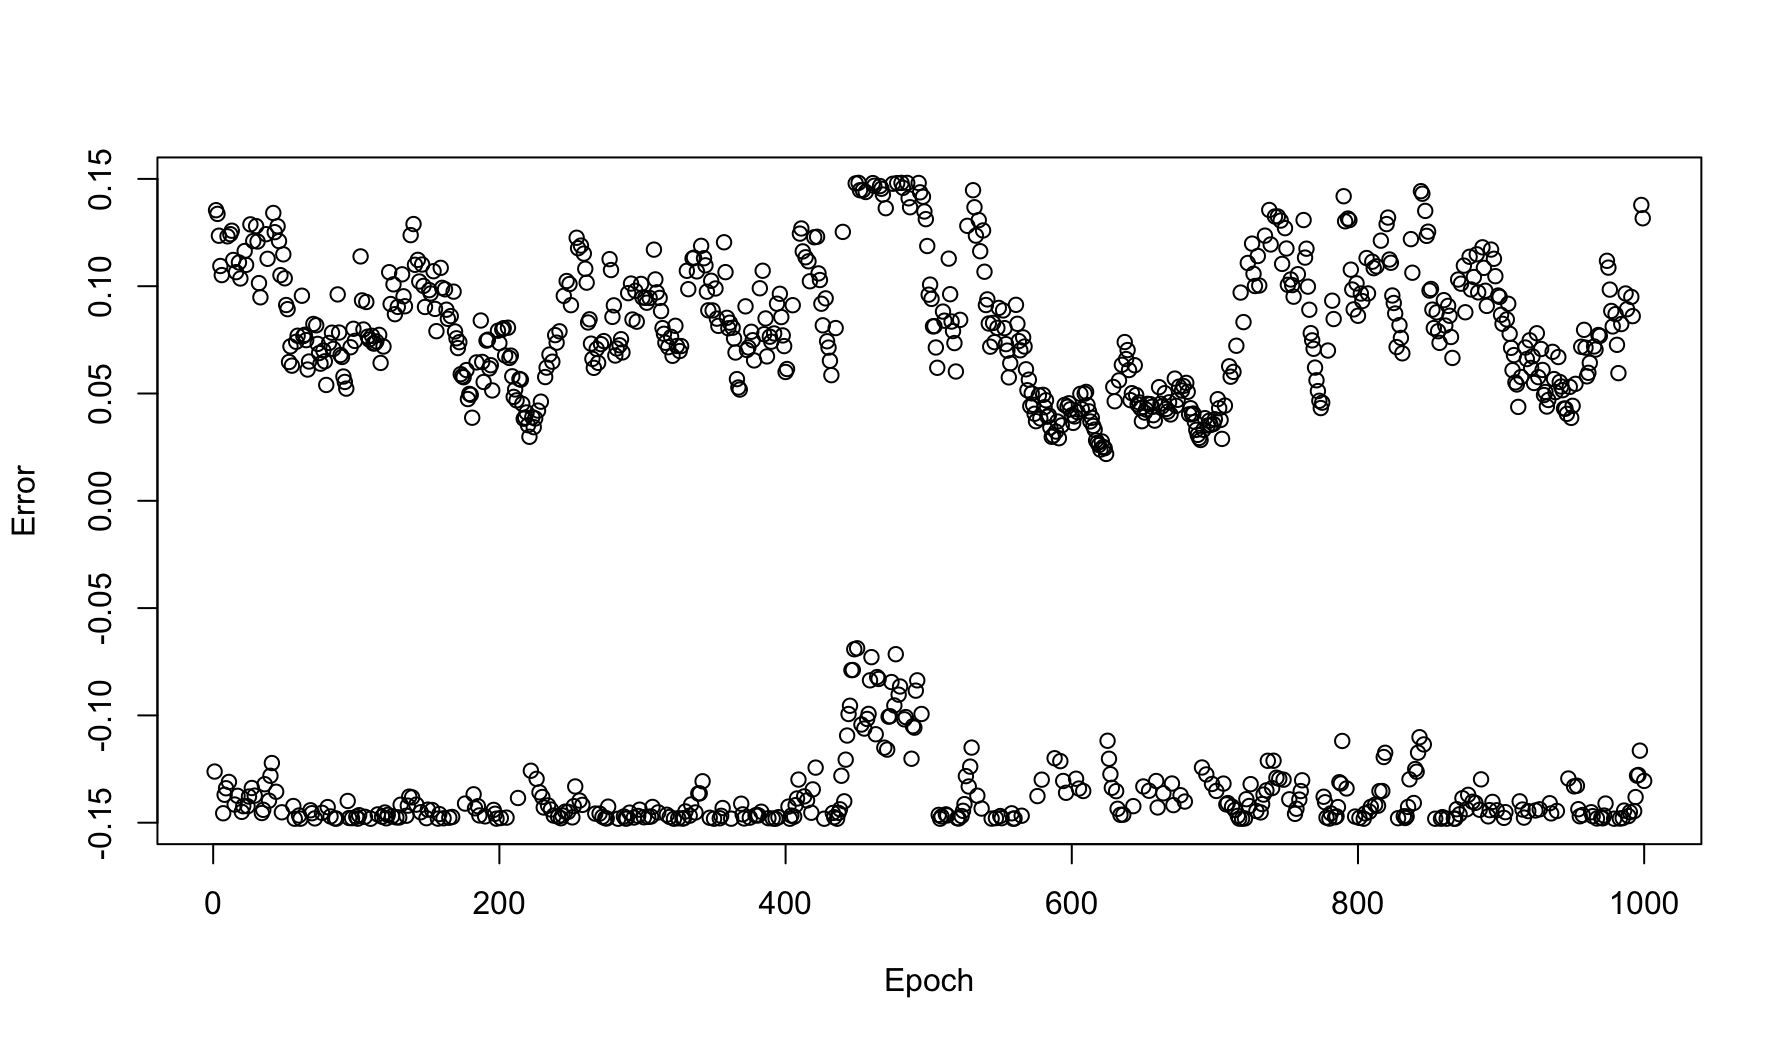
\includegraphics[width=\linewidth]{error.png}
        \caption{Error per Epoch Graph}
        \label{fig:epoch}
    \end{figure}

\section{Genetic Programming Technical Specification}
\subsection{GP Structure}

\begin{itemize}
    \item Population size: 100
    \item Number of generations: 50
    \item Crossover rate: 0.7
    \item Mutation rate: 0.08
    \item Max Depth: 4
\end{itemize}

\subsection{Graphical Representation}
The graphical representations obtained from `output.csv` are generated after each epoch (generated by GP.cpp).
    \begin{figure}[H]
        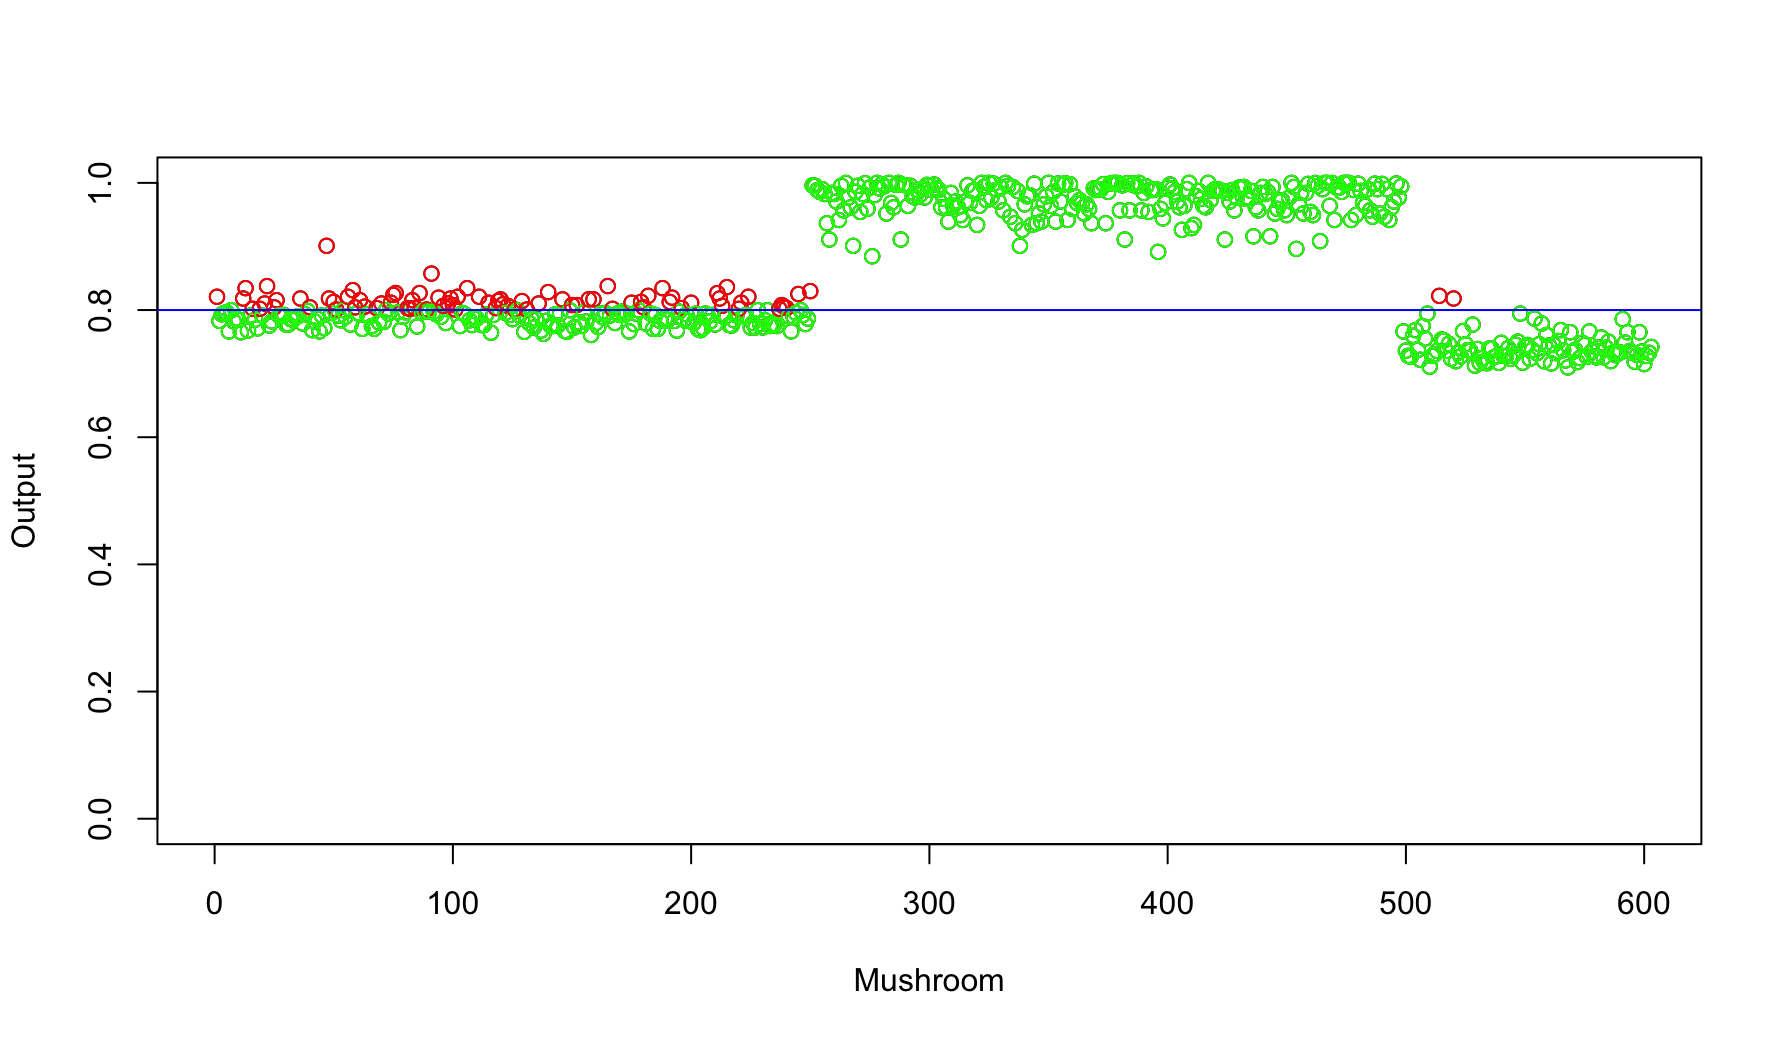
\includegraphics[width=\linewidth]{GP_scatterplot.png}
        \caption{Scatterplot of the expected data versus the GP output. The red dots represents errors.}
        \label{fig:ils}
    \end{figure}

    \begin{figure}[H]
        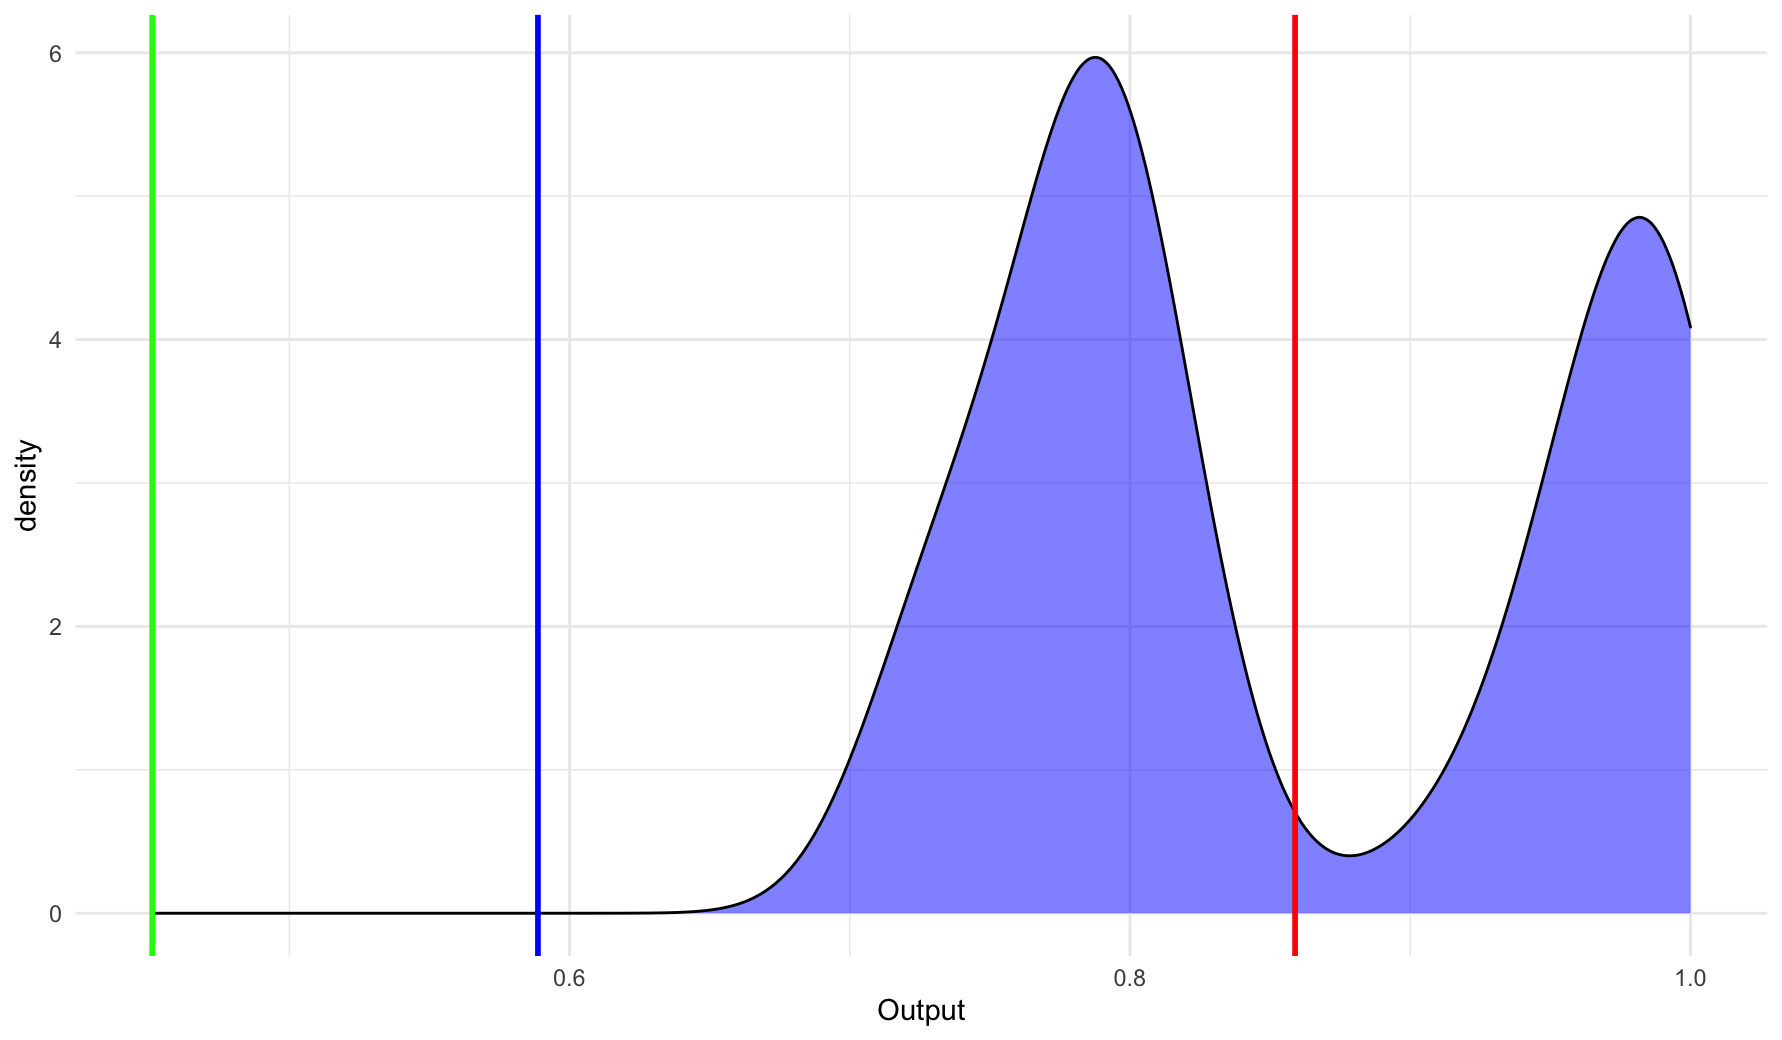
\includegraphics[width=\linewidth]{GP_density.png}
        \caption{Density Plot of the GP output. The red line gives the average output, the blue line gives the expected output, and the green line gives the actual output.}
        \label{fig:sa}
    \end{figure}

The graphical representations obtained from `error.csv` are generated after each epoch (generated by GP.cpp).
    \begin{figure}[H]
        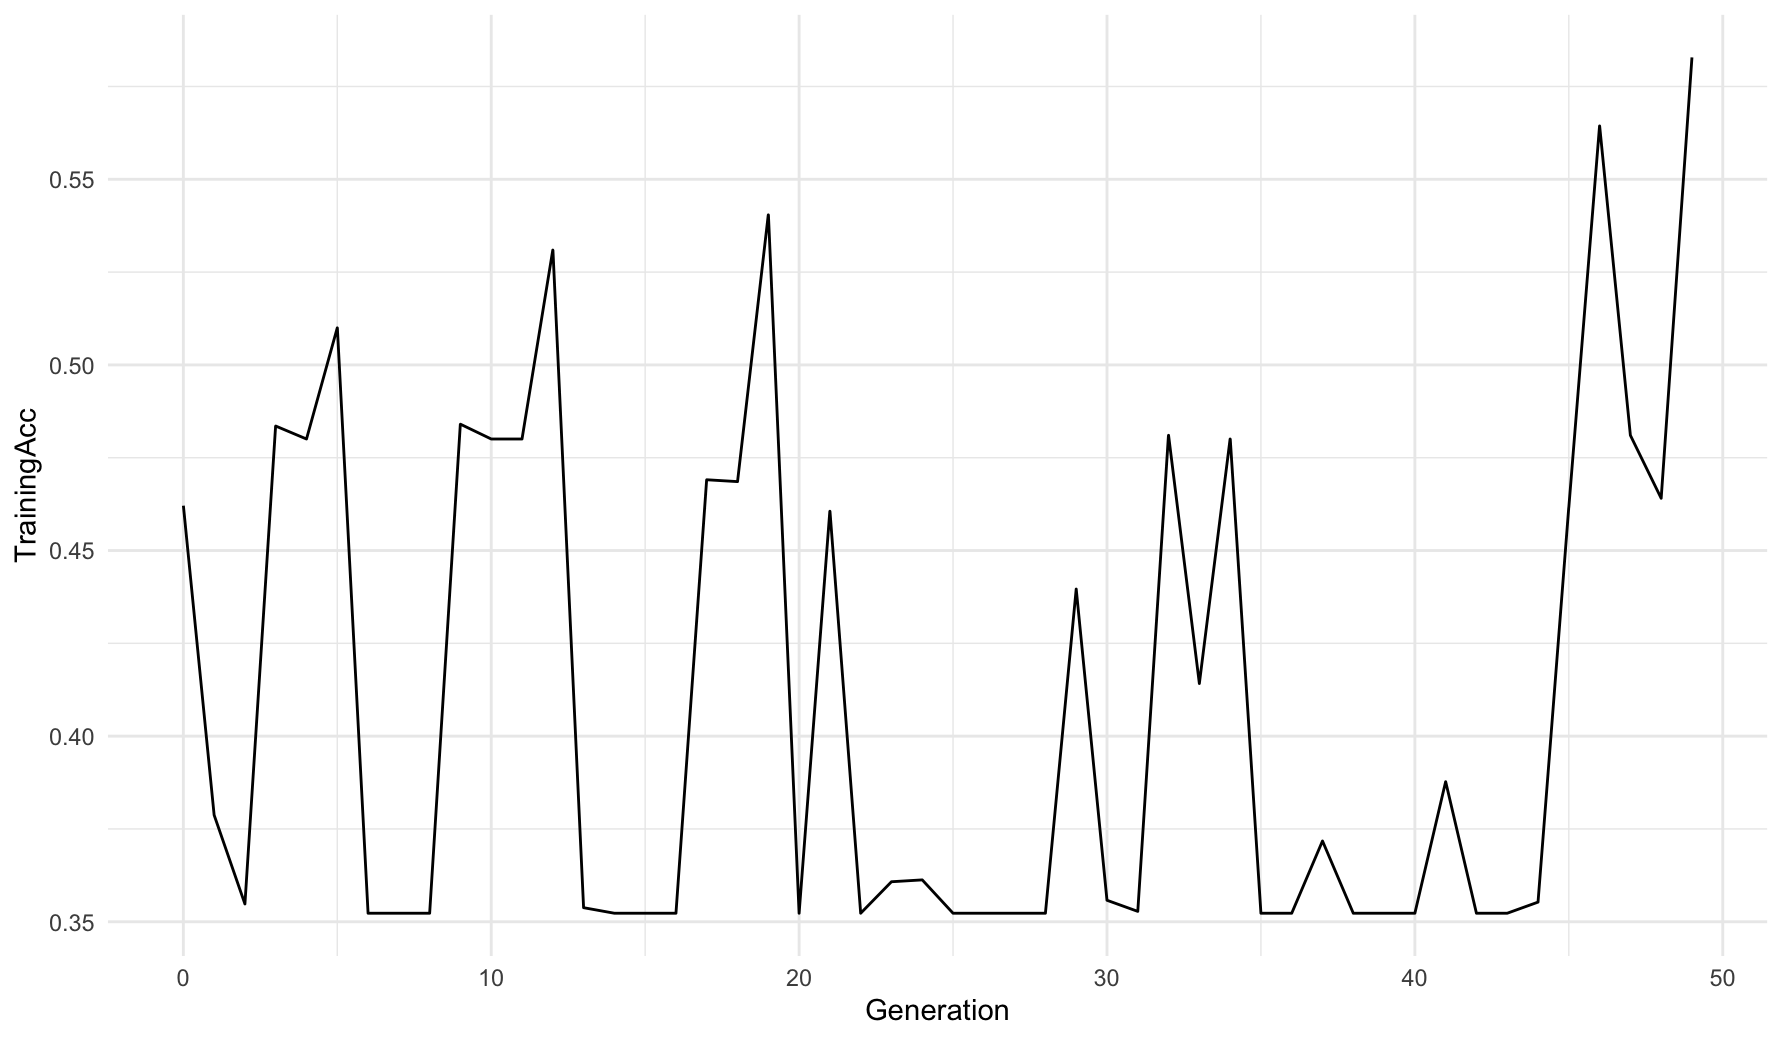
\includegraphics[width=\linewidth]{GP_trainingacc.png}
        \caption{Error per Epoch Graph}
        \label{fig:epoch}
    \end{figure}

\subsection{Critical Analysis}
The GP model provided much safer output in the sense that good mushrooms can be seen as good, and bad mushrooms can be seen as bad. The accuracy is quite high, and performs well with the test data. The model is also generalised, as it performs well with unseen data.

\end{document}

